
\documentclass[british,10pt,a4paper]{article}
\usepackage[british]{babel}
\usepackage[margin=1in, bottom=0.75in, top=0.75in, footskip=0.25in]{geometry}
\usepackage[titletoc]{appendix}
\usepackage{fancyhdr}
\usepackage{mathtools}
\usepackage[numbers]{natbib}
\usepackage{filecontents}
\usepackage{pgfplots, pgfplotstable}
    \pgfplotsset{%
    	% every tick label/.append style={scale=1.5},
        compat=newest,%
        /pgf/number format/use comma,%
        /pgf/number format/1000 sep={\,},%
        /pgf/number format/min exponent for 1000 sep=4}
\usepgfplotslibrary{statistics}
\usepackage{hyperref}
\usepackage{booktabs}
\usepackage{wrapfig}
\usepackage{listings}
\usepackage{color}
\usepackage{graphicx}
\usepackage{siunitx}
\usepackage[parfill]{parskip}
\usepackage{tikz} % To generate the plot from csv

\pgfplotsset{compat=newest} % Allows to place the legend below plot
\usepgfplotslibrary{units} % Allows to enter the units nicely

\graphicspath{ {images/} }

\setcounter{secnumdepth}{2}
\setcounter{tocdepth}{2}
\renewcommand{\arraystretch}{1.2}
\renewcommand\thesection{\arabic{section}}
\renewcommand\thesubsection{\roman{subsection}.}
\renewcommand\thesubsubsection{}
\newcommand*{\Appendixautorefname}{appendix}
\pagestyle{fancy}
\fancyhf{}
\renewcommand{\headrulewidth}{0pt}
\lfoot{Exam no: Y0076159}
\cfoot{\thepage}
\lstset{
  columns=fixed,
  breaklines=true,
  basicstyle=\ttfamily\footnotesize
  }

\usepackage[nottoc]{tocbibind}
\usepackage{csvsimple}

\begin{document}
\title{EVCO Open Assessment}
\author{Exam no: Y0076159}
\date{\today}
\maketitle
\tableofcontents
\listoffigures
\clearpage
\section{Introduction \& Problem Definition}
The game of Snake was first invented in 1976, as an arcade game named 'Blockade', and later as a computer game named 'Worms' for the TRS-80 microcomputer in 1978 \cite{Goggin2010-ao}; it gained a huge traction on mobile phones following Nokia engineer Taneli Armanto's implementation of the game for the Nokia N6110, released in 2002 \cite{Goggin2010-ao}. The game, in which a single player controls a 'snake' composed of a dot, square or object, is named after the way in which the body of the dot, square or object trails behind the dot controlled by the player. The player can turn the snake's head to change it's direction of travel, whilst the forward movement is uniform relative to time (the player has no control over the speed at which the snake moves). The player aims to win the game by collecting food places on the screen, with every item of food eaten causing the snake's tail to grow. As the player eats more food, the tail grows longer, and it becomes more difficult to navigate the plane without colliding with a surrounding wall, or the player's tail: these form the 2 losing conditions, whilst a player who successfully grows his snake to cover the entire plane has beaten the game.  \newline
\begin{figure}
	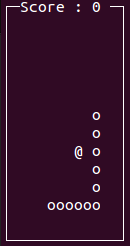
\includegraphics[width=5cm,keepaspectratio]{images/snake.png}
	\caption{A game of snake as simulated in our environment.}
	\label{fig:snake}
\end{figure}
Within the context of this project, we will be aiming to produce an evolutionary algorithm (i.e: an algorithm capable of producing a game-winning A.I. from a set of logical connectives and in-game actions) which can beat the game. That is, we will aim to maximise the number of pieces of food eaten in a run of the game. Key challenges will likely be:
\begin{itemize}
	\item To ensure the snake does not collide into it's own tail or the surrounding walls.
	\item To ensure the snake successfully eats the next piece of food without timing out.
	\item To ensure the algorithm can be run relatively quickly, so it can be evaluated over a large number of runs for statistical analysis.
\end{itemize}

\section{Literature review}
\subsection{Genetic algorithms}
Evolutionary computing is a form of algorithms which seek to find a solution to a problem through a process similar to biological evolution. \cite{Ashlock_undated-vx} The general concept involves initialising a set of candidate solutions, and iteratively updating them to obtain a 'fitter' solution. This is effectively implemented by assessing each candidate using a fitness function, before selecting a a subset of solutions which will be allowed to be bred into child solutions, mutated, and inserted into the next generation's population. This causes the overall fitness of the population to grow over the cycle of evolution, creating a candidate solution which will be closer to the global optimum. Algorithms which implement this evolutionary cycle are known as evolutionary algorithms. The field of evolutionary algorithms (EA) is sub-divided into a series of genetic representations and implementation systems. We will first discuss each of these, highlighting key papers and applications of each to our current situation.\newline

\subsubsection{Genetic algorithm}
A genetic algorithm (GA's) traditionally represent the genotype of a candidate using a binary string, although other representations are possible \cite{Whitley1994-tx}. It is extremely effective at tuning parameters of a model, as demonstrated by \citet{Wloch2004-vo} who used a GA to optimise the parameters of a simulated Formula One car, allowing it to minimise it's lap time. GA's have been implemented for use in the snake game by \citet{Yeh2016-ts}; the algorithm functioned by adjusting the rating functions of 4 operations, each of which decided the snake's next move based on either minimising the number of turns, the free space surrounding the head, or the presence of food near the snake's head. This enabled the snake to evolve a variety of solutions formed of varying frequencies of each function, resulting in a snake capable of beating the game (collecting the maximal number of food possible, where the snake's body fills the entire plane). As the snake's behaviour is not analysed by any means other than it's score in the game, it is difficult to know whether the solution reflected an EA's ability to create novel solutions to the problem. Due to this (and the restrictions on hard-coding solutions to this assessment), an approach using genetic programming was considered, as seen in \autoref{subsec:gp}.

\subsubsection{Genetic programming}
\label{subsec:gp}
Genetic programming diverges significantly from a genetic algorithm 

\subsection{Grammatical Evolution}
\subsection{Neural networks}
- GE
- Neural networks
- Co-evolution

\subsection{Applications of genetic programming to game A.I}

\subsection{General}
General research 
GP AI study 
\(https://www.gamedev.net/resources/_/technical/artificial-intelligence/application-of-genetic-programming-to-the-snake-r1175\) 

\subsection{Genetic Algorithms for snake}
\citet{Ehlis2000-sz} has provided the only comprehensive article specific to the applications of genetic algorithms to Snake. The definitions of the problem diverge from our assessment in a few non-essential ways: snake movements can be inherently defined relative to the snake's current direction (i.e: a turn\_right and turn\_left terminal is defined), and the playing field of the game is a larger rectangle than the 12\*12 field. In all other respects, \citeauthor{Ehlis2000-sz} provides
an overview of a method which functions on the same game as our case. Given this, we will first analyse this approach to the problem, and aim to build an improvement both in terms of computational performance and quality of the solution. \newline

A generic set of terminals allowing the snake to navigate the world is defined: Forward, Left and Right. The latter two allow the snake to make a change of direction relative to it's current heading, whilst the first argument does not affect the heading. The relative movement provided by the two turn operators does allow for a simpler evolution, as implementing an equivalent relative turn using absolute directions requires a significant number of operators, as we will later discuss [CITE DESIGN SECTION] \newline

Non terminals can be categorised as either food sensing (ifFoodAhead, ifFoodUp, ifFoodRight) or danger sensing (ifDangerAhead, ifDangerRight, ifDangerLeft, ifDangerTwoAhead). The use of absolute food sensing (ifFoodUp, ifFoodRight) does however require the addition of 4 sensing methods to orient the snake, allowing it to undertake the correct action given the context. This introduces some complexity into the set of operators, potentially limiting the efficiency of the algorithm.\newline

These sets of operators therefore define a generally greedy behaviour: the snake may be progressing towards the food, either at the root of the decision tree or further down once a given situation occurs (such as the 'wall-slitherer' describes in \cite{Ehlis2000-sz}). This evokes a classical approach to the game, similar to what we could expect from the average player\'s strategy. However, given that the last move of a game-winning situation would involve fully covering the map, a greedy approach would need to be very attentive to surrounding dangers to correctly navigate a path to the wall. As such, the difficulty a greedier snake may have in adapting to every potential situation may be the cause for why the algorithm may not produce optimal solutions: an example situation is stated by \citeauthor{Ehlis2000-sz}. This issue forms a basis for the design as later explained. \newline

Additional details of the algorithm are however lacking: a large population of 10000 individuals is evolved for 500 generations; the large population is potentially a counterweight to the lack of mutation, as unique genomes are created at the start of the evolution rather than during it; this most likely results in an equivalent effect. with a maximum tree size of 150 nodes to limit bloating. Crossover probability is stated as .10 for leaves, 0.80 for nodes, with a mutation probability of 0, in addition to the use of primed populations from previously unsuccessful runs. Additional details concerning which mutation or crossover functions were used are omitted, and reasonable assumptions of these are discussed in \autoref{subsec:impl} to evaluate the method. The algorithm did however account for the randomisation of food placement, mitigating it by evaluating each individual over multiple runs per generation; this was also considered in our algorithm, as we will later discuss.\newline

The proposed solution results in the creation of a game-winning decision tree (which scores the maximal 211 points). This algorithm was re-implemented to establish a benchmark for our research, revealing a significant requirement in computational time, as discussed in \autoref{subsec:impl}.


\subsection{Implementation, assumptions and results}
\label{subsec:impl}
In order to obtain benchmark fitness values, tree sizes and computational times against which to evaluate our new algorithms, the algorithm developed by \citeauthor{Ehlis2000-sz} was implemented using the Python DEAP \cite{deap} package; the code for this can be found in \autoref{app:approach1}. \newline
The algorithm was ran 20 times in order to obtain a reliable statistic of it's performance, but given the extensive computation time (20 runs at 150 generations required approximately 3 days to run using a 32 core Linux machine with 256GB of ram) required for such a large population, each run was capped at 150 generations, and was executed using the python multiprocessing module for parallel evaluation of individuals. The results of this can be extrapolated to some extent, but we will compare further algorithms on the results they achieve on the same number of generations or less. Some assumptions regarding the type of mutation (uniform tree insertion was utilised, which did not permit a variation in the mutation probability between leaf nodes and non-leaf nodes) and crossover was set with a probability of 0.0. Finally, we assumed that the fitness tournament was used to drive the fitness upwards: this was implemented with a size of 2, and that a standard evolution algorithm was used (DEAP's eaSimple, which "takes a population and evolves it in place using varAnd()).\newline
\begin{figure}
\centering
\resizebox {!} {7cm} {
	\begin{tikzpicture}[font=\LARGE]
	    \begin{axis}[xlabel=Food Eaten, ylabel=Count, ybar,xtick=,width=\textwidth]

	    \addplot+[
	    	hist={
	    		data=x,
	    		bins=14,
	    		data min = 0,
	    		data max = 134
	    	}]
	            file [y index=0]  {data/approach1.csv};
	\end{axis}
	\end{tikzpicture}
}
\caption{Histogram of best individuals from \citeauthor{Ehlis2000-sz}'s algorithm, 150 generations}
\label{fig:approach1}
\end{figure}

As seen in \autoref{fig:approach1}, the algorithm produced 8 optimal solutions (a maximal score of 133), and an average best individual of 95.38 (std: 44.24). This was achieved using an average tree size of 92 nodes. One should note that the algorithm only has a 40\% success rate in produce game-beating A.I; this is certainly related to the shortening of the algorithm by 350 generations, and the algorithm may therefore be more successful than the results above. Nevertheless, we can establish a benchmark against which we can compare future algorithms, keeping in mind the scale of resources provided to the algorithms is limited given available computing power. This can most easily be described as an average best score of 95.38 (std: 44.24), given 150 generations with a population of 10 000, with an average tree size of 92.

\section{Testing \& Design methodology}
In order to evaluate the effects of operators or fitness functions, each candidate fitness function will be evaluated 20 times, with a consistent configuration: a population of 300 individuals evolved over 150 generations. We will aim to create an algorithm which requires less computational power, and produces optimal results more consistently with a smaller population and tree size. Fitness functions will be evaluated using the same algorithm (eaSimple), although a later comparison of algorithms will be run. Finally the optimal mutation and crossover probabilities will be found by iterating combinations of them with the most promising algorithm.

\subsection{Discussion}
\section{Design \& implementation}
\subsection{Strategy}

\subsection{Fitness function}
- As we cannot implement a turn\_left and turn\_right function, detection of the direction of motion (ifMovingUp) is necessary \newline
- Why no food sensing? \newline
Cannot use steps between food picked up as food placement is too random to produce useful results.

\section{Results and analysis}
\section{Conclusion}
\subsection{Further work}
\begin{itemize}
	\item Taking a population of optimal solutions, giving them more operators and evolving a more efficient A.I. which wins the game in the smallest time possible
	\item 
\end{itemize}

\clearpage

\bibliographystyle{IEEEtranSN}
\bibliography{references}
\clearpage
\begin{appendices}

	\section{Benchmark algorithm}\label{app:approach1}
	Based on the design document by \citet{Ehlis2000-sz}. \newline
	\lstinputlisting[language=Python]{../GP/approach1.py}
  	\clearpage	

  	\section{Stream.py}\label{app:stream}
  	\clearpage

\end{appendices}
\clearpage
\end{document}
